\chapter{\uppercase{Simulation Results}} \label{chap:simulations}

This chapter provides example systems to help provide intuition into energy
shaping procedures and to demonstrate the outcome of applying energy shaping to
these example systems.
% 
Four examples are covered and they are arranged by complexity.
% 
The first example covered is the cart--spring system, which is a
single--degree-of-freedom system.
% 
This example is, perhaps, the most informative due its simplicity:
% 
with one degree-of-freedom, it is possible to provide figures demonstrating the
domain of attraction and to plot a proper phase portrait.
% 
The next example is the compass-gait biped walking down a shallow slope.
% 
This system which is motivated largely by McGeer's work \cite{McGeer1990} has
two degrees-of-freedom and exhibits conservation of energy in the continuous
dynamics.
% 
The third system is a three-link biped with a torso walking on flat ground under
the influence of \cs \cite{Spong2005} and additional
non-conservative forcing.
% 
The fourth and final system is a seven-link, multi-domain biped which uses a
number of controllers to achieve walking.
% 
This model is rather complex in comparison to the other examples and is provided
primarily to demonstrate energy shaping on multi-domain hybrid systems.

In addition to verifying the formal results guaranteed by
\thmref{theorem:main-theorem}, this chapter will also attempt to provide some
substance to the claims made about the benefits of energy shaping.
% 
It was loosely mentioned that energy shaping can be used to improve robustness
of systems with respect to perturbations in initial conditions.
% 
Although it may be possible to demonstrate the domain of attraction for some
models, doing so requires the explicit construction of a Lyapunov function.
% 
And though \thmref{theorem:main-theorem} guarantees the implicit existence of a
valid Lyapunov function by fulfilling the necessary conditions for Lyapunov's
direct method (converse Lyapunov theorem), it does not provide the explicit
function in much the same way as the definition of time-to-impact as an implicit
function does not provide any clue as to its explicit form.
% 
As a result and because of the difficulty of guessing a Lyapunov function, 




\begin{figure}[t!]
  \centering
  \def\svgwidth{0.7\columnwidth}
  \input{figs/cart_spring.eps_latex}
  \caption[Configuration of the cart--spring system.]{Configuration of the
    cart--spring system. Values used in simulation shown in \tabref{tab:cart_spring_parameters}.}
  \label{fig:cart-spring-configuration}
\end{figure}

\begin{table}[t!]
  \caption{Physical parameters for the cart--spring simulation.}
  \label{tab:cart_spring_parameters}
  \centering
  \begin{tabular}{c c c}
    $M = 1 \ \mathrm{kg},$ &
    $K = 1 \ \mathrm{N/m},$ &
    $\gamma = .2 \ \mathrm{kg/m^{2}/s}$
  \end{tabular}
  \vspace{-1em}
\end{table}

\section{Cart--Spring System}\label{sec:cart_spring}

The simplest example system to which energy shaping can be applied is a system
with a one-dimensional configuration space.
% 
The cart--spring system shown in \figref{fig:cart-spring-configuration} (with
simulation parameters given in \tabref{tab:cart_spring_parameters}) is just such
a system and can be used to build intuition into the methods presented.

\subsection{Setup}

This well-known example is highly idealized and assumes rolling without slipping
and no damping.
% 
As shown in \figref{fig:cart-spring-configuration}, the cart has mass $M$ and is
acted on by an idealized spring with stiffness $K$.
% 
It is assumed that (by turning the wheels) a force can be applied directly along
the $x$-axis in the same way in which the spring acts.

% 
Parameterizing the motion of the system by the horizontal displacement, $\q$, with
associated velocity $\dq$, leads to the configuration space $\Q = \R$ with
tangent bundle $T\Q = \R^{2}$ which has coordinates $\x = \argsqdq \in \T\Q$.
% 
Disregarding physical restrictions on spring length leads to the domain of
admissibility for the system being entire, i.e.,
\begin{align*}
  \D = \R^{2}.
\end{align*}
% 
The dynamics of the system obeys the differential equation
\begin{align*}
  M \ddq + K \q = \uu
\end{align*}
where $M$ is the mass of the cart, $K$ is the spring constant, and $u$ is the
control force in newtons.

This system is not intrinsically a hybrid system and, as a result, energy
shaping cannot be directly applied.
% 
However, this system can be made amenable to energy shaping by embedding it
in a hybrid system.
% 
Consider that the motion of the cart--spring system involves oscillation about
the origin.
% 
Thus all non-trivial trajectories pass through the origin repeatedly, so a
natural choice for the switching surface (\Poincare{} section) is the set
\begin{align}
  \Guard = \left\{ \argsqdq \in T\Q : \q = 0 \mbox{ and } \dq < 0 \right\}.
  \label{eq:cart_spring_guard}
\end{align}
% 
Using this switching surface with the domain of admissibility specified above
permits reformulation of the cart--spring system as a hybrid system:
% 
\begin{align}
  \HCS = \left\{
    \begin{array}{l l}
      \dx\hphantom{^+} = \xf\argsqdq + \xg \, \uu, & \argsqmdqm \in \D \setminus
      \Guard,\\
      \xp = \argsqmdqm, & \argsqmdqm \in \Guard,
    \end{array}\right.
\end{align}
where
\begin{align*}
  \xf\argsqdq = \left(\begin{array}{c}
      \dq\\
      -\frac{K}{M} \q
    \end{array}\right), \qquad
  \xg = \left(\begin{array}{c}
      0\\
      \frac{1}{M}.
    \end{array}\right).
\end{align*}

For the constructed hybrid system, the discrete dynamics do not have any effect
on the configuration and velocity; in other words, the discrete dynamics is the
identity map.
% 
Moreover, with no control input, the system is conservative and does not exhibit
asymptotic stability.
% 
In order to demonstrate the application of energy shaping, a limit cycle can be
induced in the system using, for example, the same dissipation present in the
Van der Pol oscillator (see \cite[pp.~13]{Khalil2002}).
% 
As described in \chapref{ch:energy-shaping}, the state of the system can be
augmented to include a storage function for energy flow due to non-conservative
forcing, i.e.,
\begin{align*}
  \x = \argsqdqW
\end{align*}
where $\W$ is an energy storage function as in \eqref{eq:storage-function-Fnc}.
% 
Applying the feedback control law
\begin{align}
  \label{eq:spring_cart_vdp_controller}
  \uu = \vv\argsqdq = \gamma(1 - \q^{2}) \, \dq + w
\end{align}
with $\gamma \in \Rnn$ leads to the hybrid control system
\begin{align}
  \label{eq:hcs_cart_spring}
  \HCSbar = \left\{
    \begin{array}{l l}
      \dx\hphantom{^+} = \xfbar\argsqdq + \xgbar \, w, & \argsqmdqm \in \D \setminus \Guard,\\
      \xp = \Delta\argsqmdqm, & \argsqmdqm \in \Guard,
    \end{array}\right.
\end{align}
where the nominal controller is subsumed under the system dynamics and energy
flow is tracked in the $W$ coordinate, viz.
\begin{align}
  \label{eq:FGbar_cart_spring}
  \xfbar\argsqdq = \left(\begin{array}{c}
      \dq\\
      -\frac{K}{M} \q + \frac{1}{M} \gamma(1 - \q^{2}) \, \dq\\
      \gamma(1 - \q^{2}) \, \dq^{2}
    \end{array}\right), \qquad
  \xgbar\argsdq = \left(\begin{array}{c}
      0\\
      \frac{1}{M}\\
      0
    \end{array}\right),
\end{align}
and the reset map acts to reset the stored energy, i.e.,
\begin{align*}
  \Delta\argsqdq = (\q, \dq, 0).
\end{align*}
% 
The hybrid control system \eqref{eq:hcs_cart_spring} is of the same form as
\eqref{eq:hcs_bar} but is written in a more compact way.


\begin{figure*}[htp!]
  \centering
  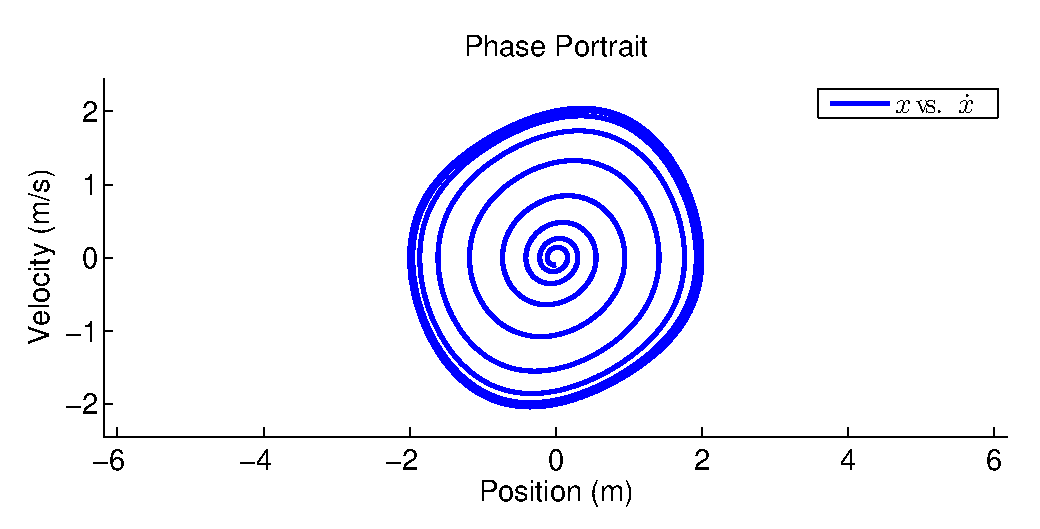
\includegraphics[width=0.85\textwidth]{hybrid_cart_spring_phase_portrait}
  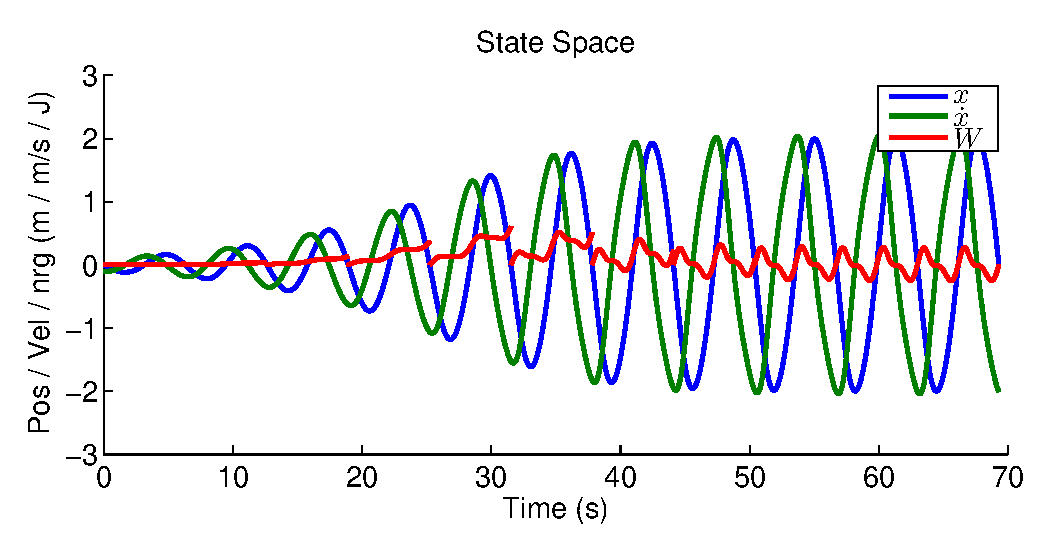
\includegraphics[width=0.85\textwidth]{hybrid_cart_spring_coordinates}
  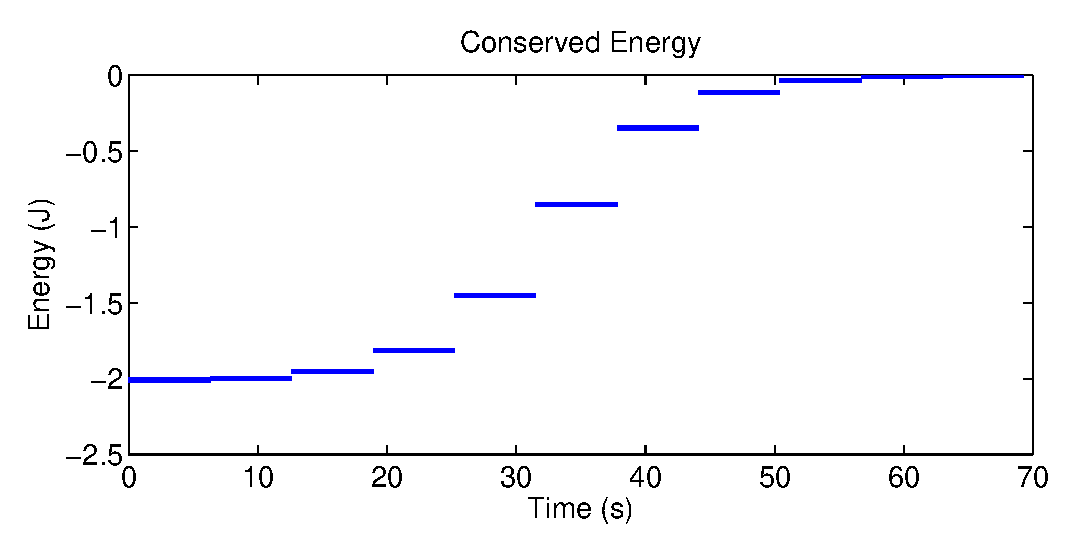
\includegraphics[width=0.85\textwidth]{hybrid_cart_spring_energy}
  \caption[Simulation of the nominal cart--spring system.]{Simulation of the
    nominal cart--spring system.
    % 
    A force from the nominal control law \eqref{eq:spring_cart_vdp_controller}
    acts on the cart.
    % 
    Top: phase portrait demonstrating the existence of a limit cycle;
    % 
    middle: evolution of the state coordinates;
    % 
    bottom: the conserved energy jumps when the storage function is reset at the
    switching surface.}
  \label{fig:cart_spring_simulation_nominal}
\end{figure*}


\subsection{Simulation of Nominal System}
Beginning from the (post-reset) initial condition
\begin{align*}
  \argsqdqW = (0, -.1, 0),
\end{align*}
a simulation was conducted to illustrate the nominal behavior of cart--spring
system governed by \eqref{eq:hcs_cart_spring} and \eqref{eq:FGbar_cart_spring}
under influence of the Van der Pol controller defined in
\eqref{eq:spring_cart_vdp_controller} with $w = 0$;
% 
that is, the closed-loop hybrid system
\begin{align}
  \label{eq:hs_cart_spring_nominal}
  \HSbar = \left\{
    \begin{array}{l l}
      \dx\hphantom{^+} = \xfbar\argsqdq, & \argsqmdqm \in \D \setminus \Guard,\\
      \xp = \Delta\argsqmdqm, & \argsqmdqm \in \Guard,
    \end{array}\right.
\end{align}
% 
The parameters used are given in \tabref{tab:cart_spring_parameters}; two of the
parameters refer to the mass and spring constant as shown in \figref{fig:cart-spring-configuration}.
% 
The simulation was designed to terminate when the distance between successive
crossings of the \Poincare{} section \eqref{eq:cart_spring_guard} dropped below
a threshold---in this case, $10^{-3}$---thus serving as the convergence
criterion.
% 
Mathematically, this convergence criterion can be expressed as
\begin{align}
  \label{eq:cart_spring_convergence}
  \P_{\TI\arx}\arx - \x < 10^{-3}, \quad \x \in \Guard.
\end{align}
% 
In this case, the distance metric is the standard Euclidean one and involves
only the velocity coordinate due to the definition of the \Poincare{} section
\eqref{eq:cart_spring_guard}.

From \figref{fig:cart_spring_simulation_nominal}, it is apparent that the
simulation lasted just under $70$ seconds.
% 
The phase portrait in \figref{fig:cart_spring_simulation_nominal} shows that the
system eventually converges to a limit cycle over relatively large number of
steps (i.e., iterations of the \Poincare{} first return map).
By counting the jumps in the plot of conserved energy in
\figref{fig:cart_spring_simulation_nominal}, one can see that convergence based
on the aforementioned criterion requires 11 ``steps'';
% 
in other words, the cart passes through the origin from the positive side 11
times.


From the evolution of the coordinates shown in
\figref{fig:cart_spring_simulation_nominal}, it is apparent that the
oscillations grow until the system reaches the limit cycle.
% 
The conserved energy of the limit cycle (as defined in
\eqref{eq:ncsys-nrg-cons} and \eqref{eq:storage-function-Fnc}) can be seen to change between iterations in \figref{fig:cart_spring_simulation_nominal}.
% 
This jump is a result of the resetting of the storage function, $W$, which
occurs when the cart passes through the switching surface
\eqref{eq:cart_spring_guard}.

\subsection{Simulation of Shaped System}

To demonstrate the effect of energy shaping, a simulation was conducted on the
cart--spring system described in the previous subsection.
% 
The relevant hybrid control system for the application of energy shaping is
given in \eqref{eq:hcs_cart_spring} and \eqref{eq:FGbar_cart_spring}.
% 
In contrast to the nominal simulation, this simulation was conducted with $w$
given by the min-norm control law \eqref{eq:min-norm} designed to satisfy the
conditions of energy shaping \eqref{eq:es-qp}, which results in the
hybrid system
\begin{align}
  \label{eq:hs_cart_spring_es}
  \HSbar = \left\{
    \begin{array}{l l}
      \dx\hphantom{^+} = \xfbar\argsqdq + \xgbar \, \mueps\argsqdqW, & \argsqmdqm \in \D \setminus \Guard,\\
      \xp = \Delta\argsqmdqm, & \argsqmdqm \in \Guard,
    \end{array}\right.
\end{align}
with $\xfbar$ and $\xgbar$ as given in \eqref{eq:FGbar_cart_spring}.

The results of the simulation of \eqref{eq:hs_cart_spring_es} are shown in
\figref{fig:cart_spring_simulation_shaped}.
% 
Like the simulation of the nominal system, this simulation of the shaped system
\eqref{eq:hs_cart_spring_es} was designed to terminate upon convergence using
the same criterion as specified in \eqref{eq:cart_spring_convergence}.
% 
From this figure, it is immediately obvious that convergence occurs in fewer
steps than for the nominal simulation;
% 
for this shaped simulation, convergence requires three steps (count the
zero-crossings of $q$ in the middle plot of
\figref{fig:cart_spring_simulation_shaped}) and the simulation lasted under 20
seconds.
% 
In addition, it is apparent from the phase portrait that the convergence happens
very rapidly.
% 
The speed of convergence can be affected by varying the gain $\resclfparam$ of
the energy shaping controller \eqref{eq:es-qp}.

These numerical simulations show that energy shaping can provide improved
convergence properties for stable systems.
% 
However, because the Van der Pol controller is globally stable, it is not
possible to demonstrate an increase in domain of attraction;
% 
this benefit of energy shaping will be shown in the next example.


\begin{figure*}[htp!]
  \centering
  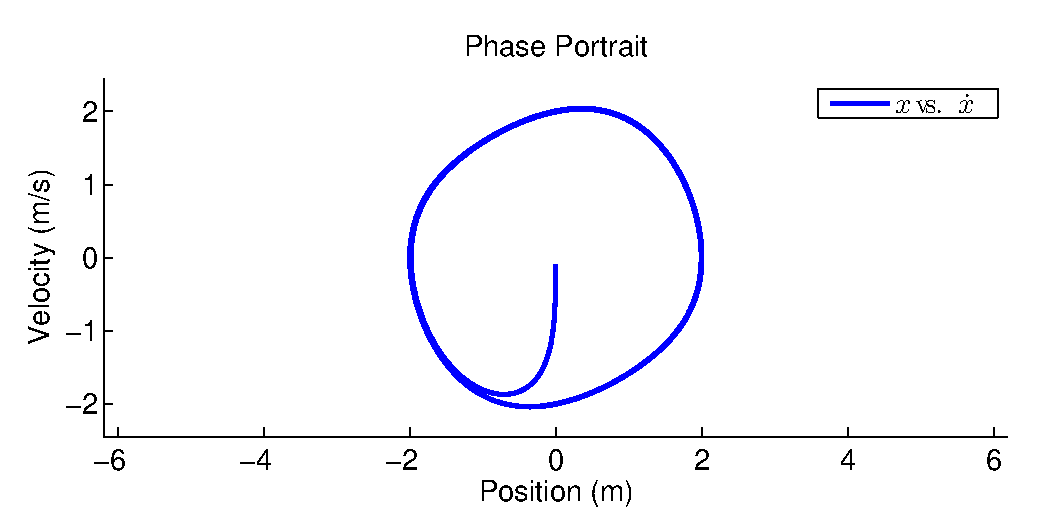
\includegraphics[width=0.85\textwidth]{hybrid_cart_spring_es_phase_portrait}
  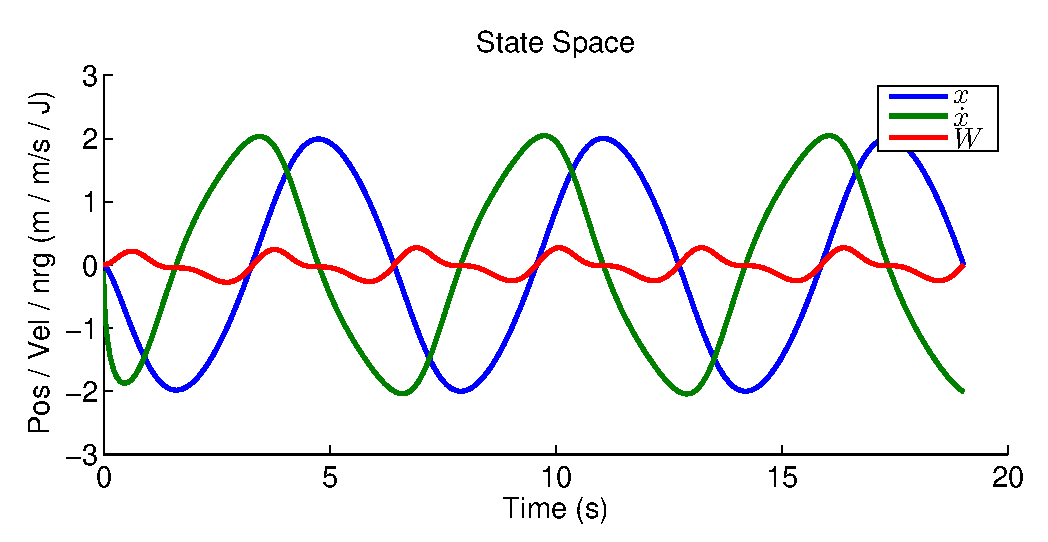
\includegraphics[width=0.85\textwidth]{hybrid_cart_spring_es_coordinates}
  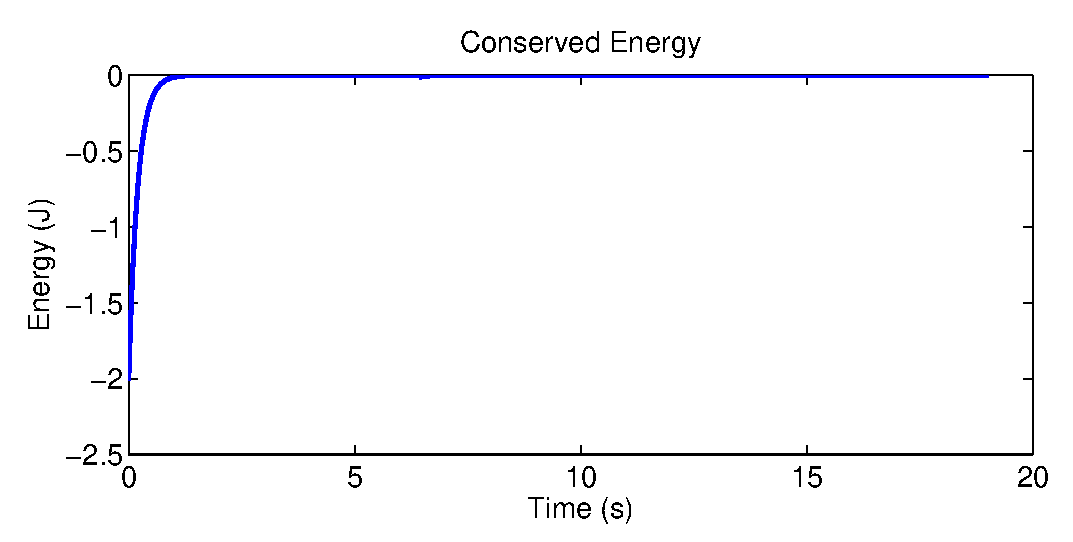
\includegraphics[width=0.85\textwidth]{hybrid_cart_spring_es_energy}
  \caption[Simulation of the shaped cart--spring system.]{Simulation of the
    shaped cart--spring system.
    % 
    A force from the nominal control law \eqref{eq:spring_cart_vdp_controller}
    acts on the cart along with a force from energy shaping.
    % 
    Top: phase portrait demonstrating the existence of a limit cycle and rapid
    stabilization;
    % 
    middle: evolution of the state coordinates;
    % 
    bottom: the conserved energy stabilizes to the desired value at an
    exponential rate.}
  \label{fig:cart_spring_simulation_shaped}
\end{figure*}


\begin{figure}
  \centering
  \def\svgwidth{0.5\columnwidth}
  \input{figs/cg2d-slope-model.eps_latex}
  \caption{Compass-gait biped with walking down a slope.}
  \label{fig:simulation-model}
  \vspace{-1em}
\end{figure}

\begin{table}[t]
  \caption{Physical parameters for the simulation model.}
  \label{tab:mparam}
  \centering
  \begin{tabular}{c c c c}
    $M =20 \ \mathrm{kg},$ &
    $m = 5 \ \mathrm{kg},$ &
    $\ell = 1 \ \mathrm{m},$ &
    $\gamma = .05 \ \mathrm{rads}$
  \end{tabular}
  \vspace{-1em}
\end{table}

\section{Compass-Gait Biped} \label{sec:simulations-compass-gait}

\begin{figure}[p!]
  \centering
  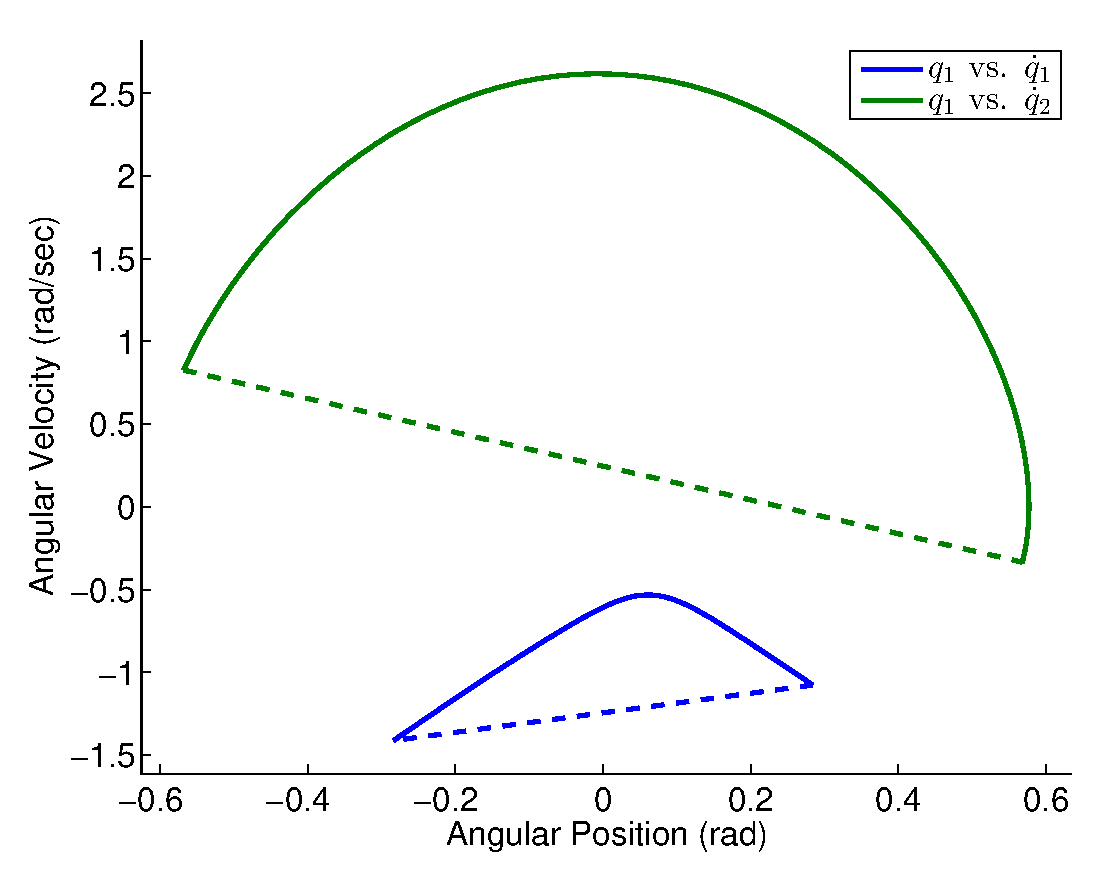
\includegraphics[width=0.75\columnwidth]{cg-limit-cycle}
  \caption{Limit cycle of the passive compass gait biped.}
  \label{fig:lc}
\end{figure}

\begin{figure}[p!]
  \centering
  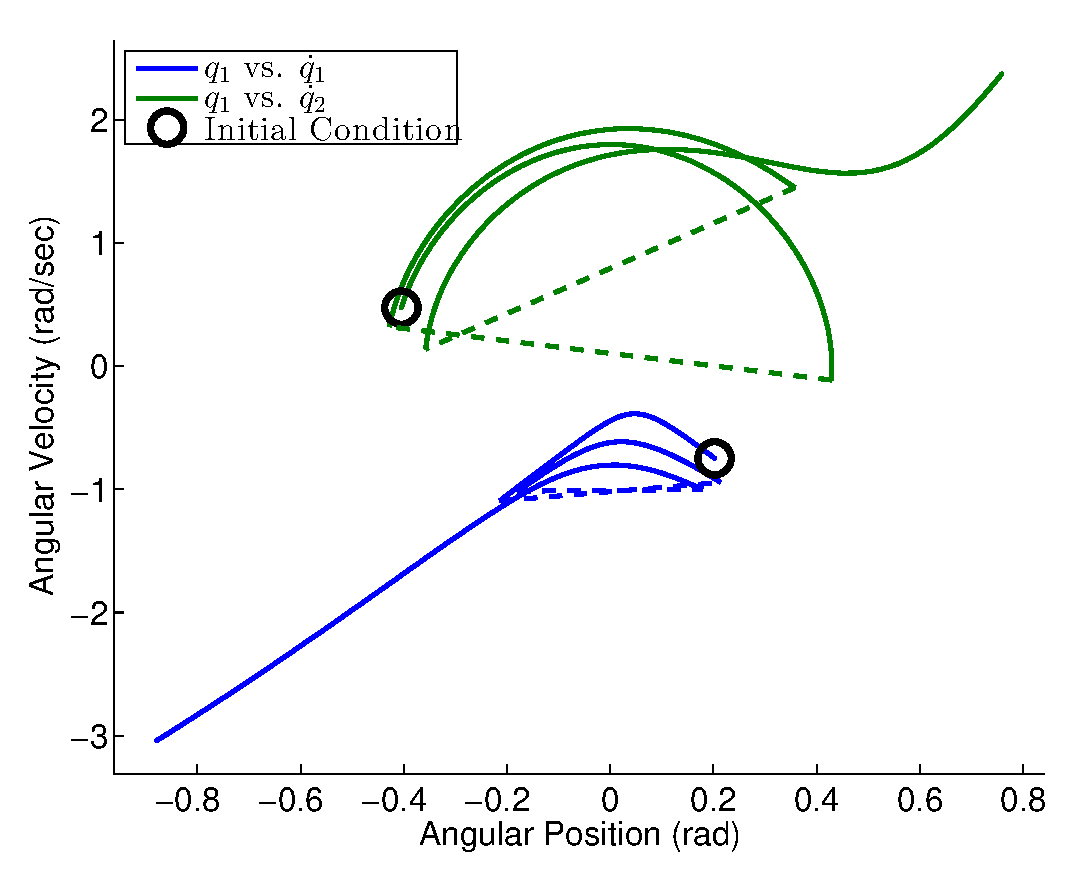
\includegraphics[width=0.75\columnwidth]{cg-pp-fall}
  \caption{The passive system cannot recover from distant states.}
  \label{fig:pp-fall}
\end{figure}

With slightly greater complexity than the cart--spring system described in
\secref{sec:cart_spring}, the compass-gait biped is a two-link rigid kinematic
chain with periodic impacts (foot-strike) which cause instantaneous jumps in the
velocity coordinates.

Using the compass-gait biped model shown in \figref{fig:simulation-model} with
parameters as shown in \tabref{tab:mparam}, simulations were conducted to
demonstrate the effectiveness of the energy shaping procedure.
% 
The limit cycle of the passive system is shown in \figref{fig:lc} with the
dotted lines representing discrete jumps from foot-strike (and coordinate
relabeling).
% 
This gait has a fixed point
% 
\begin{align}
  \label{eq:fixed-point}
  (\qst, \ \dqst) = (-0.2891, \ 0.5781, \ -1.4006, \ -0.2802)
\end{align}
% 
on the guard with eigenvalues
% 
\begin{align}
  |\lambda| = (0.5147, \ 0.5147, \ 0.0980)
\end{align}
% 
corresponding to a linearization of the \Poincare{} map restricted to the guard.
% 
Due to the restriction to the guard, the \Poincare{} section is a
codimension-one hyperplane and is thus characterized with fewer coordinates (one
fewer).
% 
Because these eigenvalues have magnitude below unity, the corresponding hybrid
periodic orbit is locally exponentially stable.
% 
The impact map can be applied to the fixed point \eqref{eq:fixed-point} to
compute the post-impact coordinates
% 
\begin{align}
  \label{eq:fixed-point-post-impact}
  \Delta(\qst, \ \dqst) = (0.2891, \ -0.5781, \ -1.0681, \ 0.6797).
\end{align}

To see the benefit of energy shaping, consider two simulations conducted from a
perturbed post-impact initial condition,
% 
\begin{align}
  \label{eq:ic-sim-1}
  (\q_{0}, \ \dq_{0}) = (0.2023, \ -0.4047, \ -0.7477, \ 0.4758),
\end{align}
% 
which was naively obtained by multiplying the post-impact fixed point
\eqref{eq:fixed-point-post-impact} by $0.7$ resulting in a relatively large
perturbation.
% 
For the passive walker, one can see from \figref{fig:pp-fall} that the biped
falls on the third step.
% 
When energy shapping is added by choosing $\frac{c_{3}}{\resclfparam} = 1$ as in
\figref{fig:pp-recover}, the biped is able to recover from the same initial
condition and quickly converges to the limit cycle.
% 

\begin{figure}[p!]
  \centering
  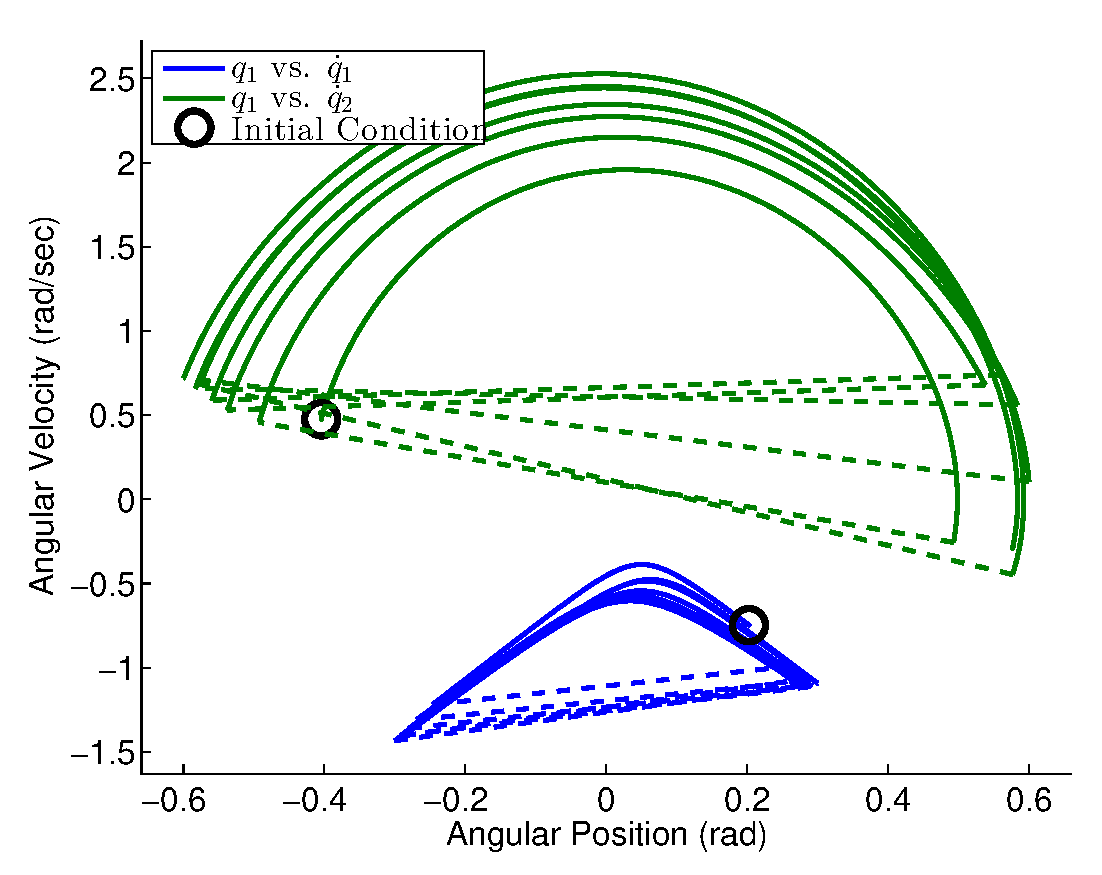
\includegraphics[width=0.75\columnwidth]{cg-pp-recover}
  \caption{Energy shaping allows recovery from more distant states.}
  \label{fig:pp-recover}
\end{figure}

\begin{figure}[p!]
  \centering 
  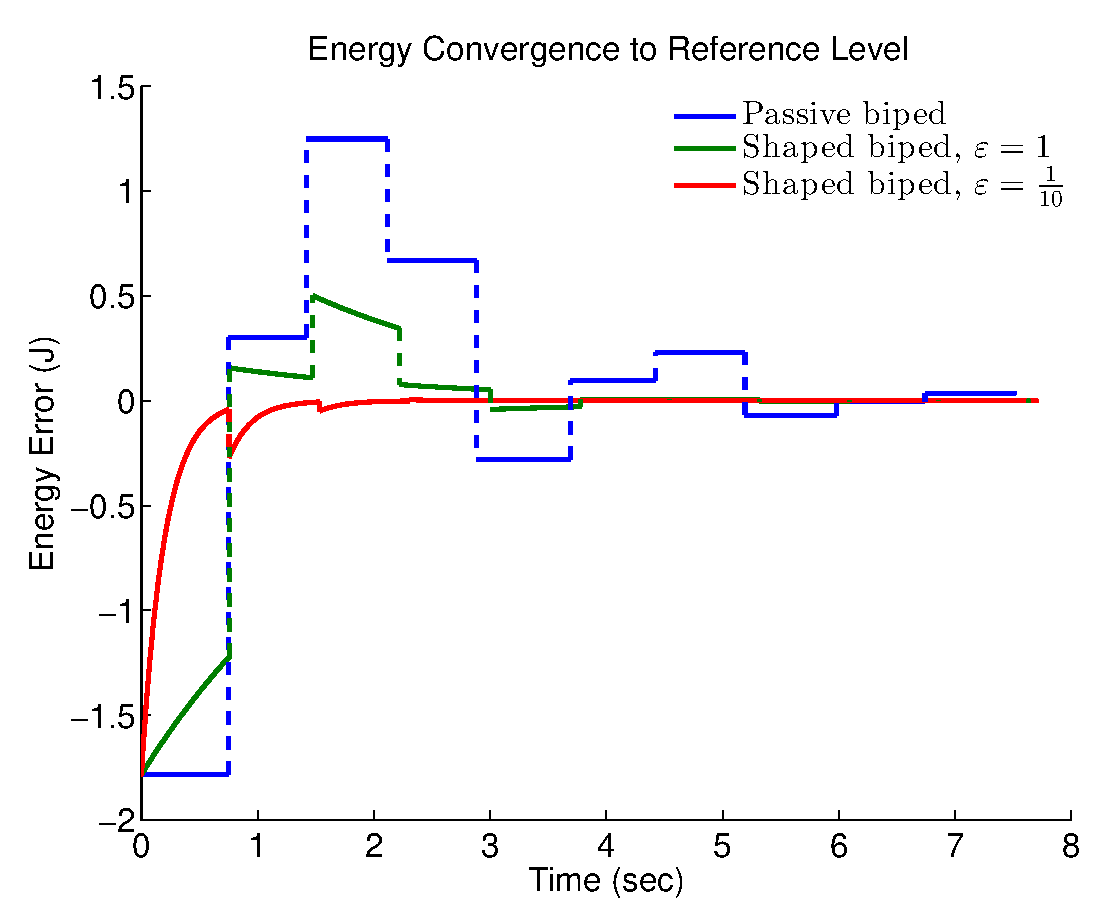
\includegraphics[width=0.75\columnwidth]{cg-energy-comp}
  \caption[Convergence has more desirable behavior with energy
  shaping.]{Convergence has more desirable behavior with energy shaping. Smaller
    values of $\resclfparam$ offer better convergence.}
  \label{fig:energy-comp}
  \vspace{-1em}
\end{figure}

In addition to the ostensible increase in robustness, energy shaping also seems
to improve convergence properties.
% 
To see this, a simulation was conducted from the starting point
% 
\begin{align}
  (\q_{0}, \ \dq_{0}) = (0.2457, \ -0.4914, \ -0.9079, \ 0.5777),
\end{align}
% 
which, in similarity to the previous simulation, was obtained by multiplying \eqref{eq:fixed-point-post-impact} by $0.85$.
% 
This point had to be closer than \eqref{eq:ic-sim-1} in order to fall within the domain of attraction (DOA) of the passive biped.
% 
The difference in convergence for the energy levels of the passive and shaped
systems is shown in  \figref{fig:energy-comp}.
% 
One can see that the shaped system converges more quickly than the passive
system.
% 
Whereas the passive system changes energy only through impact, the shaped system
also converges during the continuous dynamics.
% 
Finally, it seems, stability is mainted for large values of $\resclfparam$,
smaller values will result in better convergence so a trade-off naturally
arises.


\begin{figure}[t!]
  \centering
  \centering
  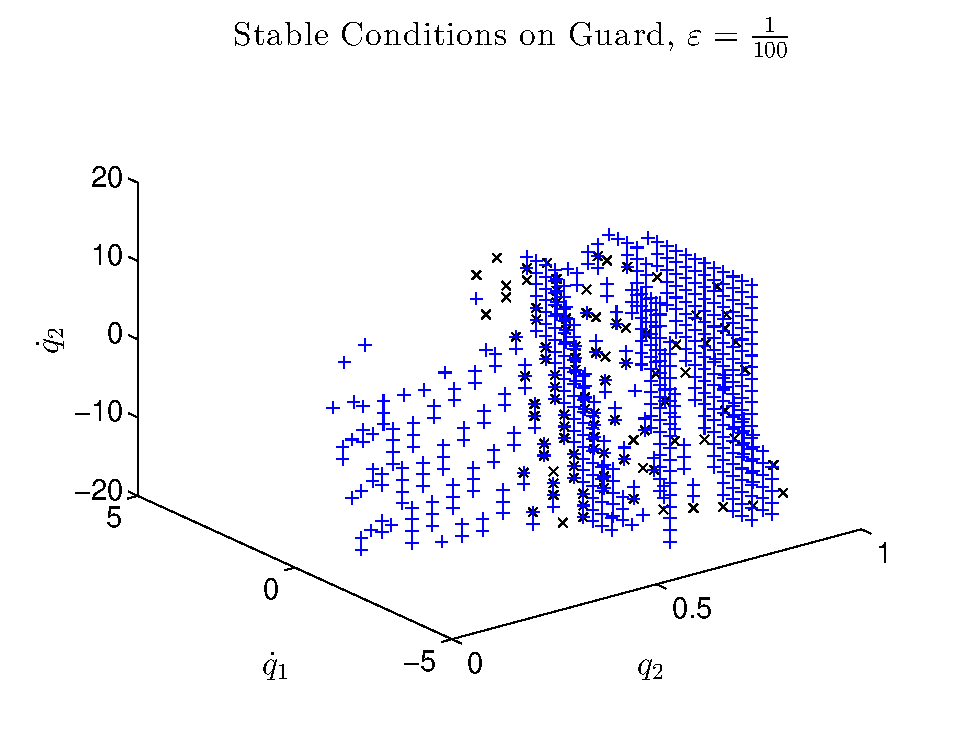
\includegraphics[width=0.75\columnwidth]{cg-poincare-cloud}
  \caption[The domain of attraction restricted to the guard.]{The domain of
    attraction restricted to the guard.
    % 
    The DOA can be viewed in three dimensions with careful scrutiny.
    % 
    The blue ``+'' symbols represent stable points of the shaped system and the
    black ``x'' symbols represents stable points of the passive system.}
  \label{fig:point-cloud}
  \vspace{-1em}
\end{figure}

More comprehensive evidence for the expansion of the domain of attraction can be
seen in \figref{fig:point-cloud} which provides a comparison of the stable
region on the guard for both the passive and shaped systems.
% 
It is interesting to note that the domain of attraction expands most readily
into the region of low energy (small steps, small angular velocities) for which
states the passive biped would simply lack the energy necessary to fall into a
gait.

\section{Seven-Link Biped}

\begin{figure}
  \centering
  \def\svgwidth{0.5\columnwidth}
  \input{figs/cg2d-7link-model.eps_latex}
  \caption{Seven-link biped configuration.}
\end{figure}

\begin{table}[t!]
  \begin{center}
    \caption[Physical model parameters of the seven-link biped.]{Physical model
      parameters of the seven-link biped. Masses and lengths are given in
      kilograms and meters, respectively.}
    \label{tab:reduction:model-parameters}
    \begin{tabular}{|c|c|c|c|c|c|}
      \hline
      $M$ & $m_{t}$ & $m_{c}$ &
      $m_{f}$ & $w_{f}$ & $w$\\
      \hline
      20 & 5 & 1 & .1 & .08 & .10 \\
      \hline
    \end{tabular}\\[.1em]
    \begin{tabular}{|c|c|c|c|c|c|c|c|c|}
      \hline
      $\ell$ & $\ell_{t}$ & $\ell_{c}$ &
      $r_{a}$ & $r_{f}$ & $r_{h}$ & $r_{t}$ & $r_{T} $\\
      \hline
      1 & .175 & .375 & .1 & .139 & .0625 & .25 & .075\\
      \hline
    \end{tabular}
  \end{center}
\end{table}


\subsection{Domain Structure}

By convention, the phases are numbered such that the transition from the last
domain to the first domain (i.e., $4 \to 1$) corresponds to heel strike as this
event signifies that the stance and swing legs should be swapped.\todo{Finish
  this section.}\xspace
% 
For the proper choice of gains, the walking controllers applied in this example
can generate a gait for which the hybrid dynamics $h_{1}(\q) = p_{stt}^{z}(\q)$,
where $p_{stt}^{z}(\q)$ is height of the stance toe above the ground, can be
combined to construct the constraint vector $H_{1}(\q, \dq, u)$. 
% 
After impact, it is desired that the stance knee be locked, that the stance foot
be flat on the ground, and that the swing toe remain fixed to the ground.
% 
These requirements dictate an apropos choice of kinematic constraints for
constructing a Jacobian for the impact map \eqref{eq:model:impact_generic}.
% 
Using toe strike as the transition leads to the switching surface
$\GuardTransition{1}{2}$ given in \eqref{eq:model:guardgeneric}.
% 

\subsubsection{Phase 2 -- Toe Lift ($tl$).}
% 
As the stance foot experiences heel roll from the previous phase and the toe
rolls into the ground causing an impact, the stance foot enters a state of flat
foot contact while the swing toe remains on the ground.
% 
The system continues under these conditions until the vertical constraining
force on the back (swing) toe reaches zero, at which point, the ground is no
longer undergoing a force interaction with the toe.
% 
This force thus represents a holonomic constraint on the system which can be
used to define both the switching surface and domain of admissibility (which
must always be checked).
% 
As the force reaches zero, the toe leaves the ground and, as there is no impact,
there is no impulsive change in momentum and thus the reset map simplifies to
the identity map, as previously mentioned.

\subsubsection{Phase 3 -- Knee Lock ($kl$).}
% 
After the swing toe lifts, the biped continues to locomote with flat foot
contact between the stance foot and the ground until the swing knee reaches full
extension, resulting in an impact which locks the knee.
% 
The locking and unlocking of knees could be accomplished by solenoid actuators.
% 
Unlike Phases 1 and 2, which are comparatively short, the biped spends a major
part of the gait in Phase 3.
% 
This ends up being useful as one could say the biped has full actuation in this
phase.
% 
The constraints imposed on the system in this domain actually reduce the
available degrees of freedom in the mechanical configuration to the same as the
number of actuators.
% 
Thus the robot can be made to move anywhere within the domain of admissibility
providing the appropriate constraints aren't violated.

\subsubsection{Phase 4 -- Heel Strike ($hs$).}
The locking of the stance knee which represents the transition to this domain
means that both knees are locked in this domain, but the system still has full
actuation.
% 
This phase ends when the swing heel strikes the ground, resulting in a
transition back to the first phase.
% 
A coordinate transformation can be constructed to ``swap'' the angles of the
stance leg and swing leg.
% 
For the model presented, the new joint angles are given by the following map:
% 
\begin{align*}
  \lefteqn{\mathcal{T}_q : (q_8, q_7, q_6, q_5, q_4, q_3, q_2, q_1)}\\
  && \mapsto (q_1, q_2, q_3, q_4, q_5, q_6, q_7, q_8).
\end{align*}
%% 
By choosing the reference frame to be on the torso, the transformation for the
base coordinates is simply the identity map.
% 
The transformation can then be written as a linear map, $\mathcal{T} =
\blockdiag(I_{6}, {\mathcal{T}_q})$ which induces pushforward $\mathcal{T}^*$.
% 
The post-impact state is thus given, as in \eqref{eq:model:impact_generic}, by
$\blockdiag({\cal T}, {\cal T}^*) \cdot \DeltaTransition{4}{1}$.
% 
Finally, it should be noted that there are certain choices of control which
could result in a bi-periodic orbits due to poor control design.

\subsection{Control Design}

The gait considered in this simulation requires the use of several different
control laws.
% 
For the sake of obtaining a passivity-based feel, \csx was taken as the basis
for sagittal control design.
% 
When combined with a spring--damper (\PD) controller to stabilize the torso,
\csx can produce stable walking gaits on point foot models under the assumption
of full actuation.
% 
This is essentially equivalent to a model with trivial foot behavior, i.e.,
either flat ground contact or no contact.
% 
In order to get nontrivial foot action, additional \PDx controllers can be added
at the ankles and at the non-stance knee.
% 
Finally, in order to avoid scuffing, which occurs when the swing toe strikes the
ground before desired, a controller is designed to rotate the toe away from the
ground with a torque that fades exponentially with the toe's distance from the
ground.

\subsubsection{CS}
\Cs, introduced in \cite{Spong2005}, works by shaping the potential energy a robot
to that of a passive biped walking down a slope.
% 
A group action effectively ``rotates the world'' by operating on the potential
energy allowing for walking on flat ground given passive walking down a slope.
% 
The goal is to combine \csx with other control laws to achieve stable walking in
the 2D sagittally-restricted kneed biped with feet.

To rotate gravity, consider the group action
\begin{align*}
  \Psi_\gamma\argsq : (p_{st}^x, p_{st}^z, \phi_{st}^{y},
  \qs^{1} - \gamma, \qsn{2}, \ldots, \qsn{6}) \longmapsto (p_{st}^x, p_{st}^z,
  \phi_{st}^{y}, \qsn{1} \ldots, \qsn{6})
\end{align*}
for slope angle $\gamma \in \S$ and define the feedback control law
\begin{align*}
  \Krg\argsq:= \G_{\qs}\argsq - \G_{\qs}(\Psi_{\gCS}\argsq)
\end{align*}
with $G_{\qs}\argsq = \pd{U}{\qs}\argsq$ which in the vector fields
\begin{align}
  \label{eq:frig}
  \frig\argsqdq = \fri\argsqdq + \gri\argsqdq \, \Krgi\argsq,
\end{align}
for $i \in \{1, \ldots, 4\}$.

\subsubsection{Spring--Damper Controllers}

Motivated by the elasticity the human ankle and by human ankle torque (see
\cite{Au2009}), \PDx controllers are considered as a means of meeting specific
control objectives.
%
For a given joint $j$ with angle $\qsn{j}$ and angular velocity $\dqsn{j}$, a
typical \PDx controller takes the form
\begin{align}
  \label{eq:upd}
  u_{\mathrm{\PD}, j}\argsqdq = -k_{j} (\qsn{j} - \qsn{j,0}) - c_{j} \,
  \dqsn{j}.
\end{align}
%
In order to stabilize the torso, \eqref{eq:upd} requires modification:
\begin{align*}
  u_{\mathrm{\PD}, \qsn{4}}\argsqdq = -k_{T} (\phi_{st}^{y} - \vartheta_{T,0}) - c_{T} \,
  \omega_{st}^{y},
\end{align*}
where $\phi_{st}^{y}$ is an Euler angle for the torso and $\omega_{st}^{y}$ is
the body-fixed angular velocity of the torso in the sagittal plane for the model
described earlier.
%
The controller is applied at the swing hip, $\qsn{4}$.
%
To have the swing foot land in a desirable configuration, and motivated by
measurements of human ankle torque during walking, the \PDx controller
\eqref{eq:upd} is applied at $\qsn{6}$.
%
Heuristics has shown that a \PDx controller at the stance ankle may often
contribute to stability and thus \eqref{eq:upd} is used at $\qsn{1}$.
%
In order to get the swing knee moving forward after heel strike, it was
necessary to impose \eqref{eq:upd} on $\qsn{5}$.

For simplicity take these controllers to be a set on each domain $i$ such that
\begin{align*}
  U_{\gSD}^{i} = \left\{
    \begin{array}{l @{\hspace{2em}} l}
      \{1, 4, 5, 6\}, & i = 1,\\
      \{1, 4, 6\}, & i = 2, 3, 4.
    \end{array}\right.
\end{align*}
One can observe that the controllers are continuous through a single step with
the exception of the controller designed for the swing knee.
%
In a continuous time system, this would mean the torques for smooth control laws
would be smooth, but in a hybrid system with impulse-like forces due to impacts,
discontinuities will occur in the velocities causing jumps in those control laws
which depend on these variables.
%
The keen observer might notice that if equivalent controller parameters were
found for $\qsn{1}$ and $\qsn{6}$, these controllers could be replaced by actual
spring--damper mechanisms.
%
These controllers can be combined to construct
\begin{align*}
  \Krti\argsqdq := \sum_{j \in U_{\gSD}^{i}} u_{\PD, j}\argsqdq
  \cdot b_{\qs, j},
\end{align*}
where $b_{\qs, j}$ is the $j$\textsuperscript{th} basis vector for the coordinates $\qs$.
%
Applying these controllers to \eqref{eq:frig} gives
\begin{align}
  \label{eq:frigt}
  \frigt\argsqdq = \frig\argsqdq + \gri\argsq \Krti\argsq,
\end{align}
where gains (\tabref{tab:pdgains}) are lumped into superscripts.

\begin{table}[t!]
  \begin{center}
    \caption{Gains for seven-link biped simulation.}
    \label{tab:pdgains}
    \begin{tabular}{|c|c|c|c|c|c|c|c|}
      \hline
      $k_{1}$ & $c_{1}$ & $\qsn{1, 0}$ & $k_{T}$ & $c_{T}$ & $\qn{T, 0}$ &
      $\gSP_{1}$ & $\gCS$\\
      \hline
      30 & 0.1 & -0.5 & 100 & 5 & 0 & 10 & 0.05 \\
      \hline \hline
      $k_{5}$ & $c_{5}$ & $\qsn{5, 0}$ & $k_{6}$ & $c_{6}$ & $\qsn{6, 0}$ &
      $\gSP_{2}$ & $g$ \\
      \hline
      70 & 1 & 0.5 & 30 & 1 & 0 & 20 & 9.81\\
      \hline
    \end{tabular}
  \end{center}
\end{table}

\subsubsection{Scuffing Prevention Controller}

In order to avoid the scuffing phenomenon, a controller can be designed which
repels the swing toe from the ground.
%
To minimize interference with the rest of the system's control, the scuffing
prevention controller imposes exponential spatial disipation that and thus only
makes a significant contribution when the swing toe passes near the floor.
%
This control law thus takes the form
\begin{align*}
  \Krm\argsq = -\gSP_{1} e^{\gSP_{2} \cdot p_{swt}^z\argsq} \cdot b_{6},
\end{align*}
where $\gSP_1, \gSP_2 \in \R$ are positive constants and represent the strength
of repulsion and spatial dissipation rate, respectively, $b_{\qs, 6}$ is the
6\ssth basis vector in $\qs$, and $p_{swt}^z : \Q \to \R$ is the height of the
swing toe above the ground.
%
This control law is only desirable when the swing toe is in the air, so
appropriate application leads to the following vector fields:
%
\begin{align*}
  \frigtm\argsqdq = \frigt\argsqdq +
  \left\{
    \begin{array}{l @{\hspace{1em}} l}
      \boldzero, & $i = 1, 2$,\\
      \gri\argsq \, \Krmi\argsq, & $i = 3, 4$.
    \end{array}
  \right.
\end{align*}

\subsection{Simulation of Nominal System}

Applying the feedback control laws as shown above to the hybrid control system
$\HCS$ gives the hybrid system
\begin{align*}
  \HS^{\gCS, \gSD, \gSP} = (\Gamma, \D, \Guard, \Delta, \mathcal{F}^{\gCS, \gSD,
    \gSP}),
\end{align*}
where $\mathcal{F}^{\gCS, \gSD, \gSP} = \{\frigtm\}_{i = 1}^{4}$.
%
This hybrid system was simulated with model parameters given in
\tabref{tab:reduction:model-parameters} and control parameters given in
\tabref{tab:pdgains}.
%
The joint angles and torques resulting from this walking simulation are shown in
\figref{fig:reduction-angles} and \figref{fig:reduction-torques} as dashed lines
alongside their counterparts from the later 3D simulation.
%
The stability of the gait can be examined by considering the codimension-one
\Poincare{} section $\Guard_{4}^{1}$, which is the guard of domain 4 (i.e., heel
strike) and involves switching legs.
%
To minimize the perturbations necessary to examine the \Poincare{} map, one can
perturb along a minimal set of bases that span the \Poincare{} map locally.
%
Holonomic constraints represent restrictions on the degrees of freedom of a
system and this shows up in a dropping of rank in the \Poincare{} map.
%
For this particular model, these minimal bases can be found by moving the fixed
frame to the fixed stance foot, then perturbing along angles $\qsn{3}$,
$\qsn{4}$, $\qsn{6}$ and angular velocities $\dqsn{1}$, $\dqsn{3}$, $\dqsn{4}$,
$\dqsn{6}$.
%
Because the knees are locked, $\qsn{2} = \dqsn{2} = \qsn{5} = \dqsn{5} = 0$ and
one can solve for $\qsn{1}$ such that the swing heel is on the ground.
%
Thus the \Poincare{} map for the orbit drops rank to seven.
%
Through optimization, the fixed point
\begin{align*}
  \qs^{*} &= (-.163, 0, .245, -.139, 0, -.003),\\
  \dqs^{*} &= (-.987, 0, 1.090, 1.068, 0, .067),
\end{align*}
is found.
%
A numerical approximation of a linearization of the Jacobian of the \Poincare{}
map in the seven minimnal bases yields eigenvalues with magnitudes $0.613$,
$0.169$, $0.056$, $\ldots$.
%
In general, eigenvalues with magnitudes below unity for discrete-time systems
indicate stability.
%
The \Poincare{} map for the simulated system is indeed stable thus implying
$(q^*, \dot q^*)$ is a fixed point of a stable periodic orbit which represents
the stable walking gait.

One could perform a similar analysis taking a different \Poincare{} section such
as the guard for knee lock.
%
This map has two bases more than the guard for heel strike as used above;
%
one may no longer solve for $\qsn{1}$ and $\dqsn{5}$ becomes arbitrary.
%
By taking this \Poincare{} section and performing analysis, one would find seven
non-zero eigenvalues for the reasons alluded to above.
